\chapter{Introduction}

\section{Contexte}

Dans le cadre de son travail de bachelor, l'étudiant a été mandaté par l'entreprise Breitling pour concevoir une machine permettant de mesurer la réserve de marche (RM) d’un mouvement de montre mécanique de manière accélérée.\\ 

Afin de réduire les temps de mesure et d’optimiser les ressources de production, l’entreprise souhaite mettre en place une méthode de mesure réduite, basée sur l’analyse des derniers tours de barillet uniquement. 
Cette approche permettrait de caractériser la réserve de marche de manière plus rapide.

\section{Problématique}

La mesure classique de la réserve de marche d’un mouvement mécanique consiste à laisser fonctionner la montre jusqu’à son arrêt complet après un remontage total. Cette méthode présente l’inconvénient majeur d’être très chronophage.  
Par exemple, selon le site internet de Breitling \cite{Chronomat_South_Sea}, le modèle « Chronomat Automatic 36 Swatch South Sea » dispose d'une réserve de marche de 42 heures. Ce qui signifie que la mesure de la réserve de marche de ce modèle prend au minimum 42 heures.\\

Dans un contexte industriel, ces durées de mesure élevées impliquent l’immobilisation prolongée des machines de test, ce qui oblige l’entreprise à multiplier les postes de mesure afin de maintenir un rythme de production acceptable. 
Cette situation engendre des coûts supplémentaires ainsi qu’une complexification de l’organisation des tests.

\section{Objectifs}

L’objectif principal de ce travail de bachelor est de concevoir une machine capable de mesurer la réserve de marche d’un mouvement de montre mécanique de manière accélérée, tout en conservant une précision suffisante pour une utilisation industrielle.  

Plus précisément, ce travail vise à :
\begin{itemize}
    \item concevoir un système permettant de remonter et de dévider le barillet de manière contrôlée ;
    \item proposer et intégrer un posage adaptable à différents types de mouvements ;
    \item intégrer un système de détection fiable de l’arrêt du mouvement ;
    \item proposer une solution globale reproductible et utilisable en environnement industriel.
\end{itemize}

\section{Description de l'entreprise partenaire - Breitling}

Fondée en 1884 en Suisse, Breitling est une maison horlogère de renommée mondiale spécialisée dans les montres de luxe de haute précision. 
Historiquement liée aux univers de l’aviation et de la navigation, la marque s’est imposée comme une référence en matière de chronographes professionnels.

Breitling se distingue par son savoir-faire horloger suisse, combinant tradition artisanale et innovation technologique. 
Une grande partie de ses mouvements sont certifiés chronomètres par le COSC \cite{cosc_certification}, garantissant une précision élevée. 

Aujourd'hui, la marque est présente à l'international et est représentée par des célébrités telles que le footballeur Erling Haaland \cite{Breitling_Haaland}.

\begin{figure}[H]
    \centering
    \begin{subfigure}{0.45\textwidth}
        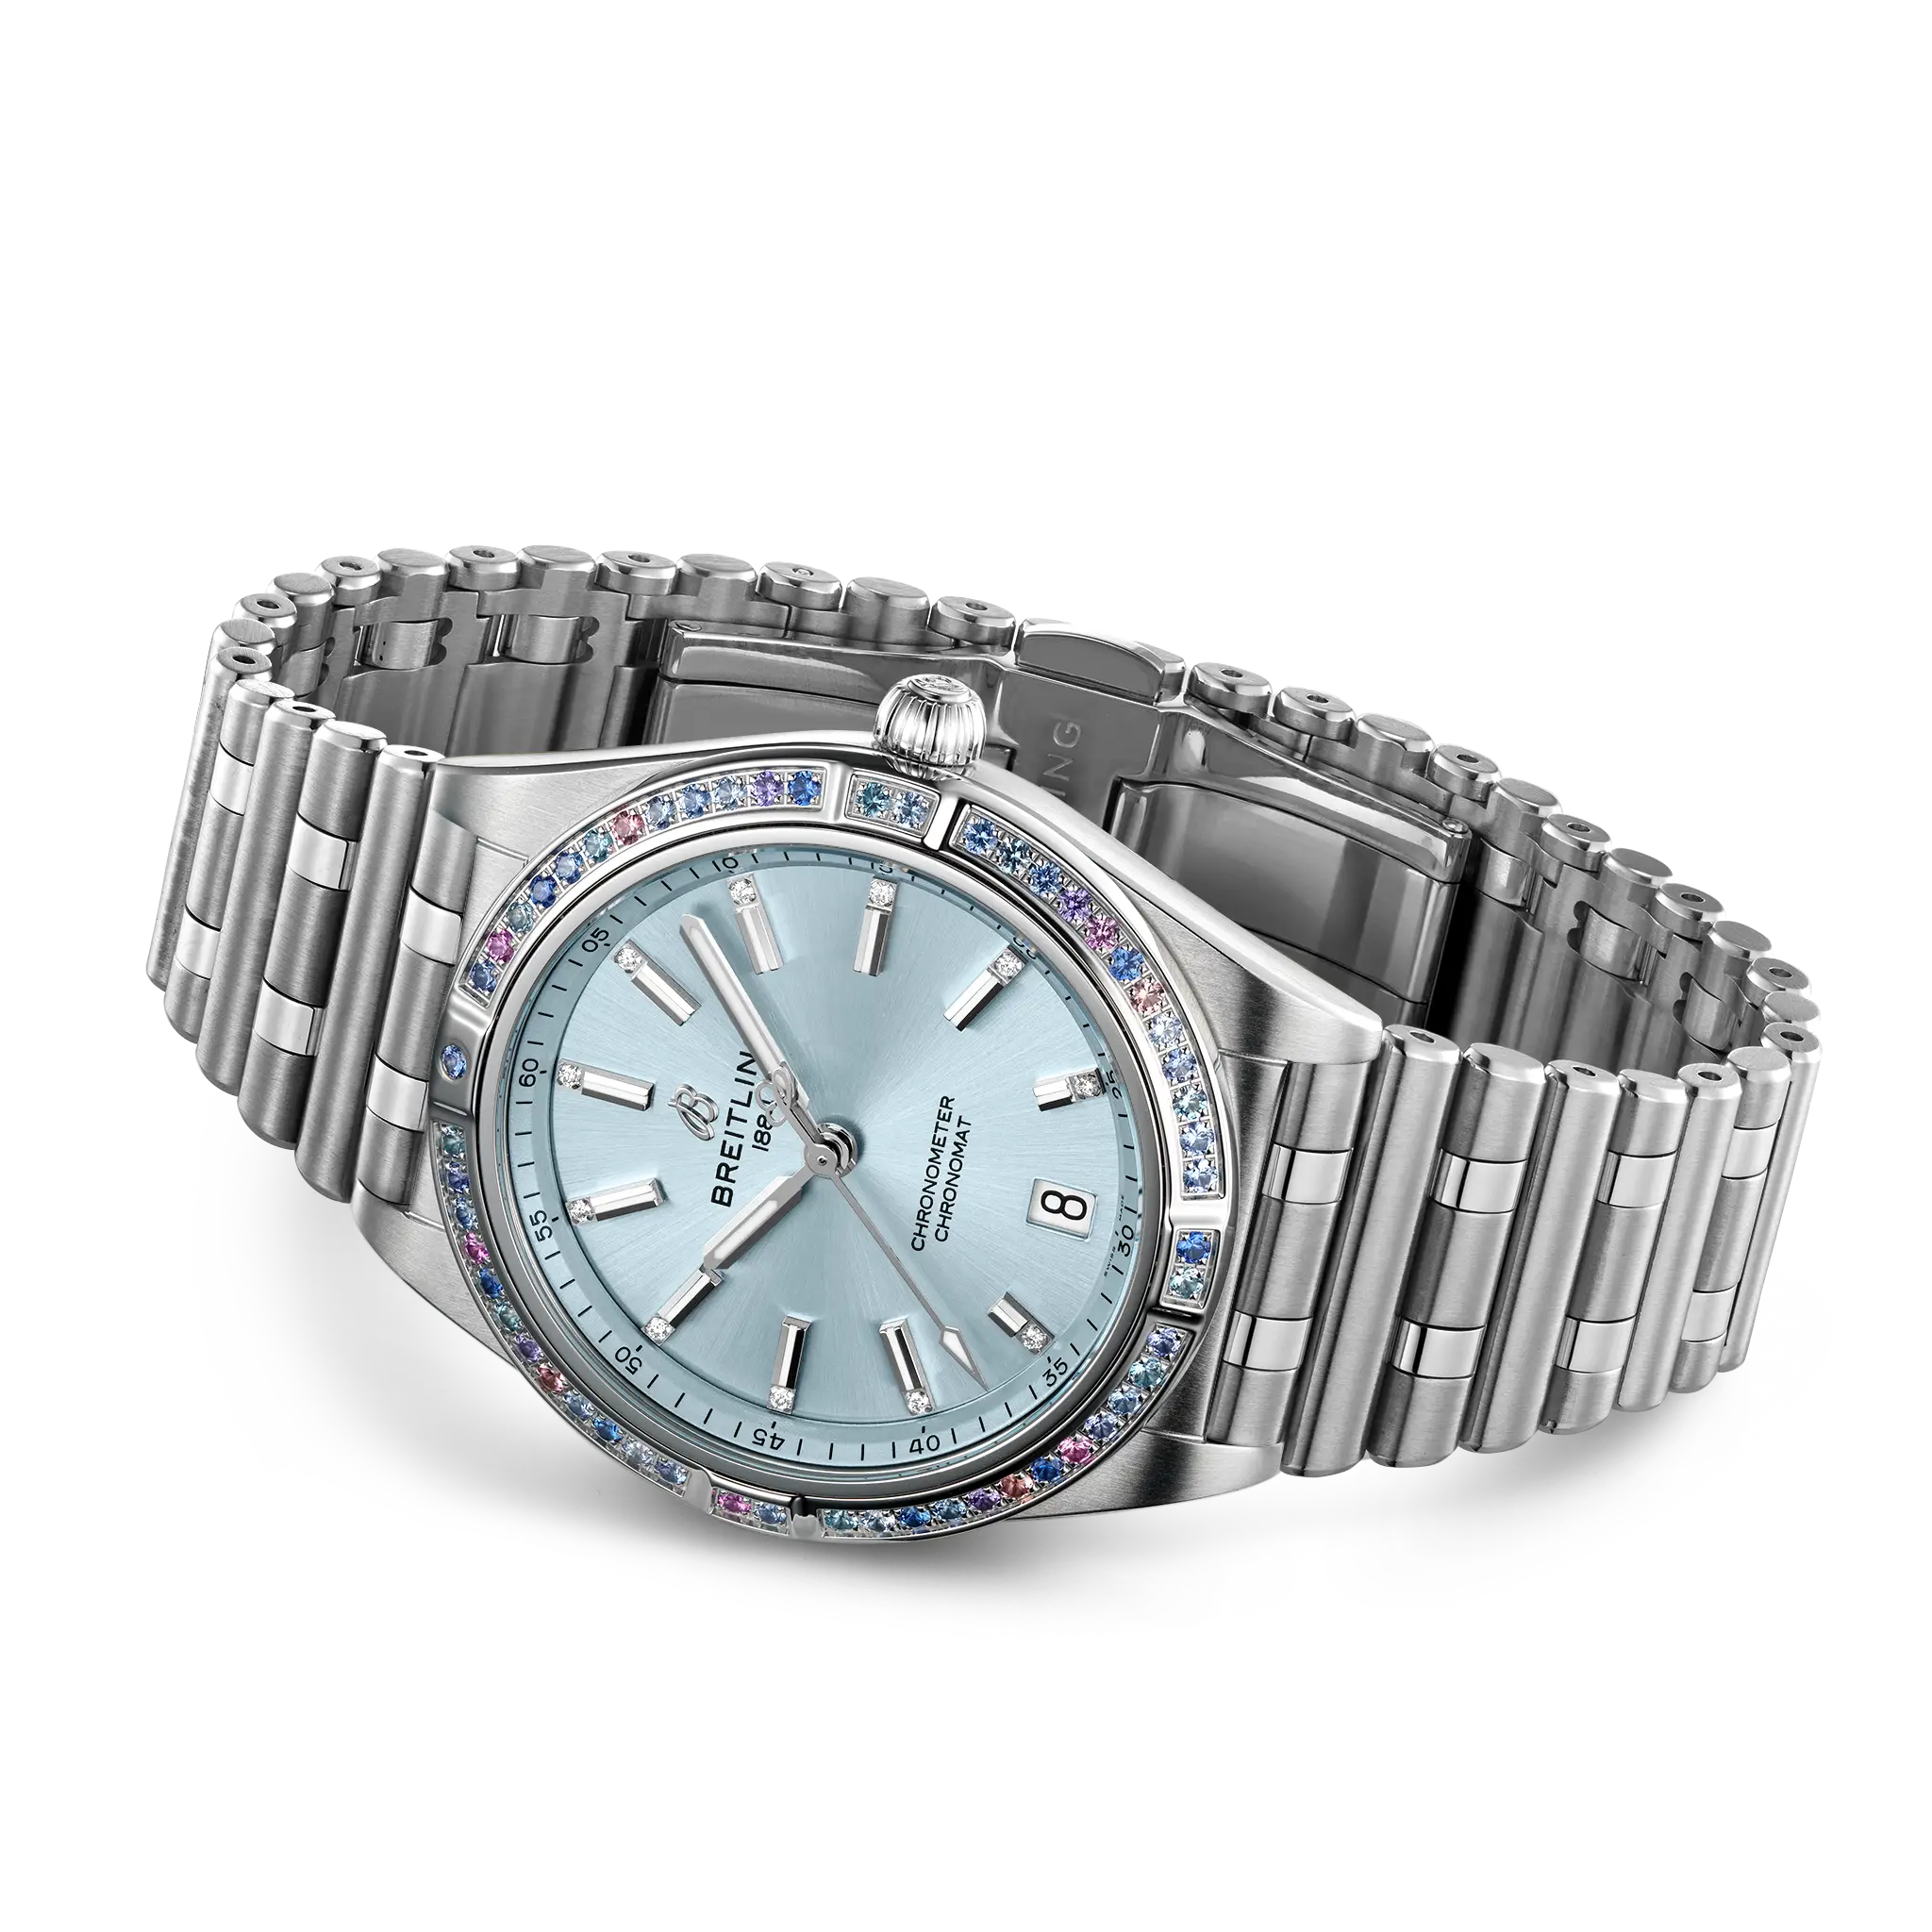
\includegraphics[width=\textwidth]{assets/figures/Introduction/Description de l'entreprise/Chronomat_Automatic_36_South_Sea_1.png}
    \end{subfigure}
    \hfill
    \begin{subfigure}{0.45\textwidth}
        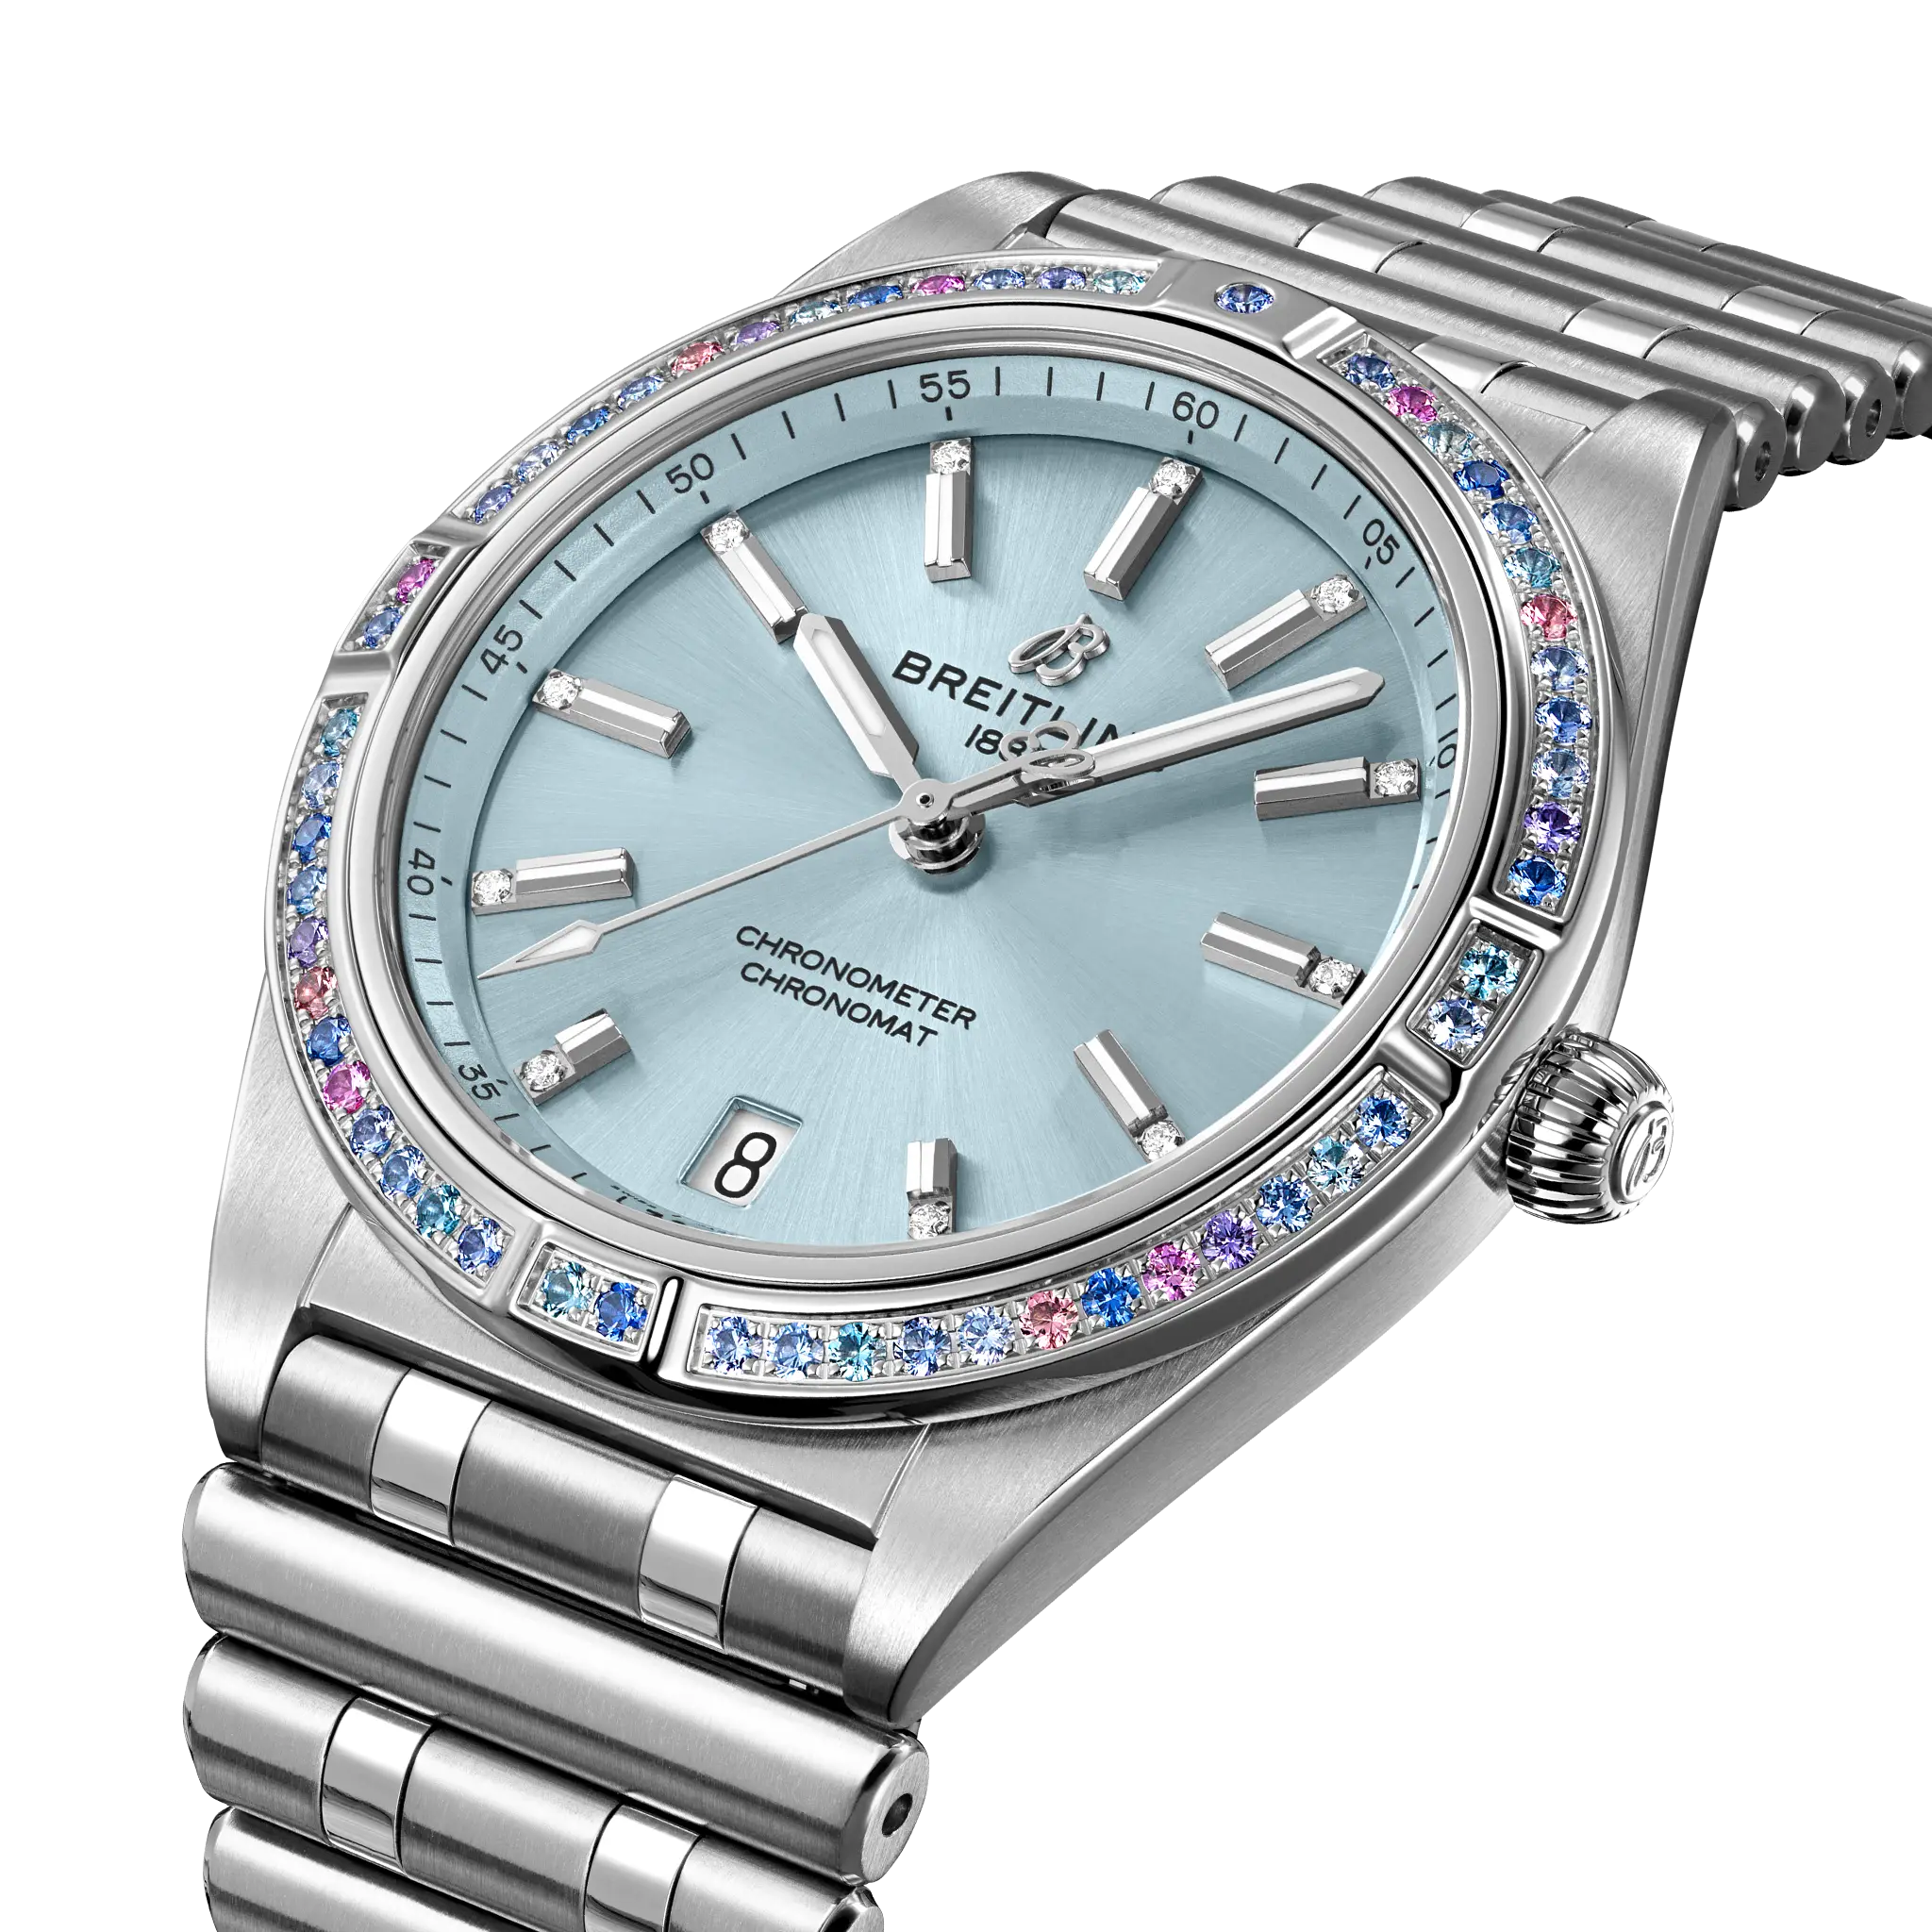
\includegraphics[width=\textwidth]{assets/figures/Introduction/Description de l'entreprise/Chronomat_Automatic_36_South_Sea_2.png}
    \end{subfigure}
\caption{Chronomat Automatic 36 Swatch South Sea \cite{Chronomat_South_Sea}}
    \label{fig:chronomat_south_sea}
\end{figure}
